
\documentclass[tikz, border=1cm]{standalone}
\usepackage{pgfplots}
\usetikzlibrary{arrows,shapes,positioning}
\graphicspath{{graphics/}}
\pgfplotsset{compat=1.18}
\definecolor{webgreen}{rgb}{0,.5,0}
\definecolor{webblue}{rgb}{0,0,.8}
\definecolor{webred}{rgb}{0.8, 0, 0}   
\definecolor{webbrown}{rgb}{.6,0,0}
\definecolor{webyellow}{rgb}{0.98,0.92,0.73}
\definecolor{webgray}{rgb}{.753,.753,.753}


\begin{document}
	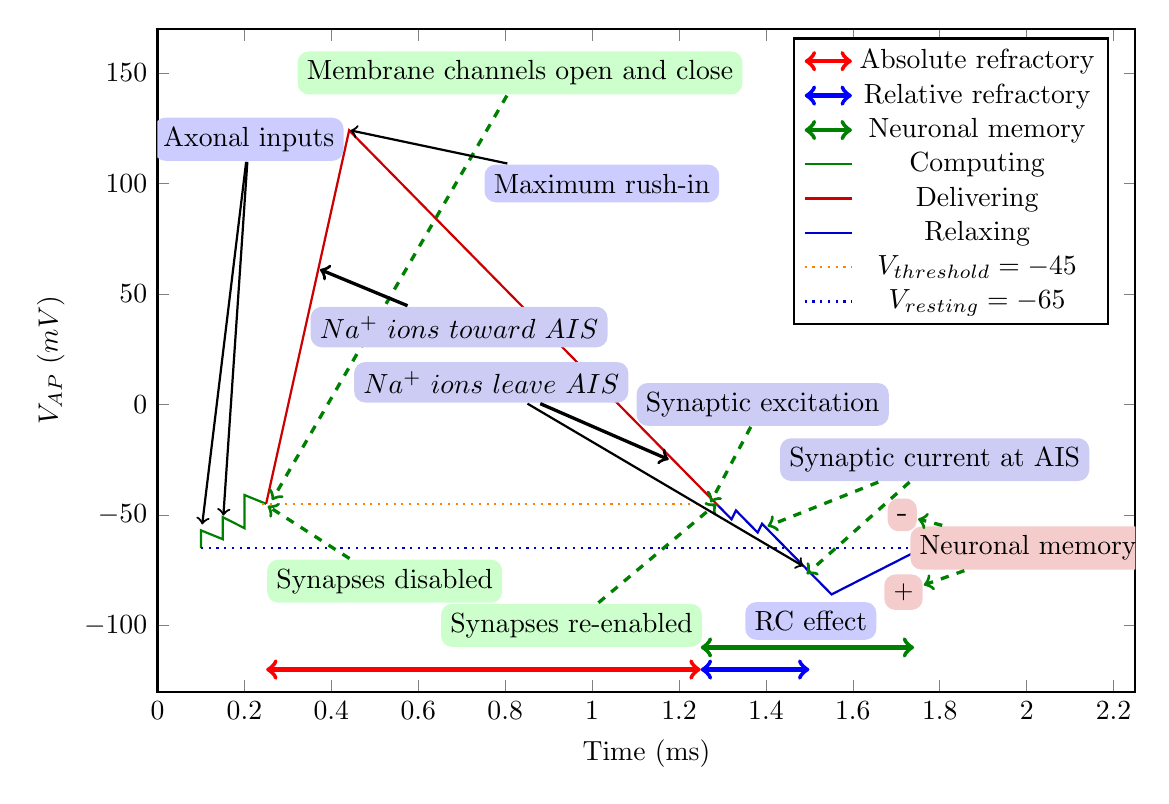
\begin{tikzpicture}
		\begin{axis}[ thick,          
		%	hide axis,
%		title = {Schematics of action potential},
			width=14cm, height=10cm,
			xmin=0, xmax=2.25,
			ymin= -130, ymax = 170,
			xlabel={Time (ms)},
			ylabel={$V_{AP}\ (mV)$},
			legend style={at={(.65,0.77)},anchor=west},
			thick
			]

\addplot [<->, red, ultra thick] coordinates {(0.25,-120)  (1.25,-120)};
  \addlegendentry{Absolute refractory}
\addplot [<->, blue, ultra thick] coordinates {(1.25,-120)  (1.5,-120)};
\addlegendentry{Relative refractory}
\addplot [<->, webgreen, ultra thick] coordinates {(1.25,-110)  (1.741,-110)};
\addlegendentry{Neuronal memory}

% The initial computation
\addplot[
webgreen, very thick,
no marks, mark=*, mark size=2, thick,
] plot coordinates {
	(0.1,-65)
	(0.1, -57)
	(0.15, -61)
	(0.15, -51)
	(0.2, -56)
	(0.2, -41)
	(0.25, -45)
};
\addlegendentry{Computing}




% The main  Action Potential schematics
\addplot[
webred, very thick,
no marks, mark=*, mark size=2, thick,
] plot coordinates {
	(  0.25,-45)
	(  0.441,124)
	(  1.291,-46)
};
\addlegendentry{Delivering}
\addplot[
webblue, very thick,
no marks, mark=*, mark size=2, thick,
] plot coordinates {
	(  1.291,-46)
	(  1.301,-48)
(  1.311,-50)
(  1.321,-52)
(  1.331,-48)
(  1.331,-48)
(  1.341,-50)
(  1.351,-52)
	(  1.361,-54)
	(  1.371,-56)
	(  1.381,-58)
	(  1.391,-54)
	(  1.391,-54)
	(  1.401,-56)
	(  1.411,-58)
	(  1.421,-60)
	(  1.431,-62)
	(  1.441,-64)
	(  1.451,-66)
	(  1.461,-68)
	(  1.471,-70)
	(  1.481,-72)
	(  1.491,-74)
	(  1.501,-76)
	(  1.511,-78)
	(  1.521,-80)
	(  1.531,-82)
	(  1.541,-84)
	(  1.551,-86)
	(  1.561,-85)
	(  1.571,-84)
	(  1.581,-83)
	(  1.591,-82)
	(  1.601,-81)
	(  1.611,-80)
	(  1.621,-79)
	(  1.631,-78)
	(  1.641,-77)
	(  1.651,-76)
	(  1.661,-75)
	(  1.671,-74)
	(  1.681,-73)
	(  1.691,-72)
	(  1.701,-71)
	(  1.711,-70)
	(  1.721,-69)
	(  1.731,-68)
	(  1.741,-67)
};
\addlegendentry{Relaxing}


%% Excitation at synapse and AIS
       \node[anchor=west, rectangle, rounded corners,fill=webblue!20] (happensA) at (axis cs:1.1,0){Synaptic excitation};      
\node (happensB) at (axis cs:1.26,-49){};
\draw[->,dashed, very thick, webgreen](happensA)--(happensB);

\addplot[
no marks, orange,thick,dotted
] plot coordinates {
	(0.24,-45)
	(1.25,-45)
};
\addlegendentry{$V_{threshold}=-45$}

\addplot[
webblue,% thick,
no marks, 
thick,dotted
] plot coordinates {
	(0.1,-65)
	(1.95,-65)
};

%\draw[orange,very thick,dotted] (0.1,-65) -- (1.95,-65);
\addlegendentry{$V_{resting}=-65$}


% The threshold potential
%\draw[blue,very thick,dotted] (0.24,-45) -- (1.25,-45);

       \node[anchor=west, rectangle, rounded corners,fill=green!20] (sourceA) at (axis cs:0.25,-80){Synapses disabled};
\node (destinationA) at (axis cs:0.23,-43){};
\draw[->,dashed, very thick, webgreen](sourceA)--(destinationA);
%
       \node[anchor=west, rectangle, rounded corners,fill=green!20] (sourceB) at (axis cs:0.65,-100){Synapses re-enabled};
\node (destinationB) at (axis cs:1.31,-41){};
\draw[->,dashed, very thick, webgreen](sourceB)--(destinationB);

       \node[anchor=west, rectangle, rounded corners,fill=webblue!20] (sourceC) at (axis cs:1.43,-25){Synaptic current at AIS};
\node (destinationC) at (axis cs:1.38,-57){};
\draw[->,dashed, very thick, webgreen](sourceC)--(destinationC);
\node (destinationCc) at (axis cs:1.47,-81){};
\draw[->,dashed, very thick, webgreen](sourceC)--(destinationCc);

       \node[anchor=west, rectangle, rounded corners,fill=green!20] (sourceD) at (axis cs:0.32,150){Membrane channels open and close};
\node (destinationD) at (axis cs:0.25,-48){};
\draw[->,dashed, very thick, webgreen](sourceD)--(destinationD);

       \node[anchor=west,  rectangle, rounded corners,fill=webblue!20] (sourceE) at (axis cs:0.35,35){$Na^+\ ions\  toward\ AIS$};
       
%       \node[anchor=west, rectangle, rounded corners,fill=webblue!20] (happensA) at (axis cs:1.1,0){Synaptic excitation};      
       
\node (destinationE) at (axis cs:0.35,63){};
\draw[->,very thick](sourceE)--(destinationE);

       \node[anchor=west, rectangle, rounded corners,fill=webblue!20] (sourceF) at (axis cs:0.45,10){$Na^+\ ions\  leave\ AIS$};
\node (destinationF) at (axis cs:1.2,-27){};
\draw[->,very thick](sourceF)--(destinationF);

%\node (destinationG) at (axis cs:1.35,-82){};
%\draw[->,thick](sourceF)--(destinationG);

\node (destinationH) at (axis cs:1.51,-76){};
\draw[->,thick](sourceF)--(destinationH);

       \node[anchor=west, rectangle, rounded corners,fill=blue!20] (sourceAx) at (axis cs:-0.01,120){Axonal inputs};
\node (destinationAxA) at (axis cs:0.10,-59){};
\draw[->,thick](sourceAx)--(destinationAxA);

\node (destinationAxB) at (axis cs:0.15,-55){};
\draw[->,thick](sourceAx)--(destinationAxB);

% Point to maximum rush.-in current
       \node[anchor=west, rectangle, rounded corners,fill=blue!20] (rushin) at (axis cs:0.75,100){Maximum rush-in};
\node (rushinA) at (axis cs:0.42,125){};
\draw[->,thick](rushin)--(rushinA);

% RC effect
       \node[anchor=west, rectangle, rounded corners,fill=blue!20] (RC_effect) at (axis cs:1.35,-98){RC effect};

\node[anchor=west, rectangle, rounded corners,fill=webred!20] (memory) at (axis cs:1.73,-65){Neuronal memory};
\node [below,left, rectangle, rounded corners,fill=webred!20] (memoryplus) at (axis cs:1.75,-50){\large -};
\draw[->,dashed, very thick, webgreen](memory)--(memoryplus);
\node  [below,right, rectangle, rounded corners,fill=webred!20] (memoryminus) at (axis cs:1.67,-85){\small +};
\draw[->,dashed, very thick, webgreen](memory)--(memoryminus);


		\end{axis}
	
\end{tikzpicture}
\end{document}
	

